
\section{Background}

\subsection{Portuguese}
\label{section:pt}

Portuguese is the mother tongue of approximately 215 million people globally, making it the sixth most spoken in the world by number of native speakers. It is the official language of seven countries and maintains co-official status in three others. The language is further divided into two main dialects that are generally mutually intelligible: European and Brazilian. The varieties of Lusophone countries in Africa and Asia often resemble their European counterpart more closely due to prolonged colonial rule, though the influence of indigenous languages and the transatlantic slave trade resulted in some shared phonological and prosodic divergence among certain African variants and Brazilian Portuguese in particular.

Similar to other Romance languages, Portuguese is characterized by moderate fusional inflection and, by consequence, a somewhat less rigid word order. While it is generally an SVO language, it also allows for SOV constructs when, for example, object pronouns are realized preverbally in what is known as proclisis. Object pronouns may otherwise be attached after the verb as an enclitic, with usage varying by dialect and context. There also exists a mesoclitic construction—restricted to verbs in the future or conditional tense—wherein a personal pronoun, object pronoun, or both may be inserted between a verb stem and its inflectional suffix.

\begin{exe}
\ex\label{pro}
\gll me\ chamo\\
{\scshape 1.sg}=call.{\scshape 1.sg.pres}\\
\glt ``(I) call myself" \citep{galves2005}

\ex\label{en}
\gll chamo-me\\
call.{\scshape 1.sg.pres}={\scshape 1.sg}\\
\glt ``(I) call myself" \citep{galves2005}

\ex\label{meso}
\gll dar-lhes-ão\\
give={\scshape dat.3.pl=3.pl.fut}\\
\glt ``(they) will give them" \citep{wetzels2018}
\end{exe}

Contractions are also ubiquitous in both written and spoken Portuguese, irrespective of register. Many common function word pairs are realized exclusively in their merged forms, analogous to French \textit{du} (de + le) and Spanish \textit{al} (a + el). A few examples of mandatorily-contracted words are provided in Table~\ref{tab:contractions}.

\begin{table}[ht]
\renewcommand{\arraystretch}{1.2}
    \centering
    \begin{tabular}{@{}c|cccc@{}}
         & \textit{o} & \textit{a} & \textit{os} & \textit{as} \\
        \hline
        \textit{a} & \textit{ao} & \textit{à} & \textit{aos} & \textit{às} \\
        \textit{de} & \textit{do} & \textit{da} & \textit{dos} & \textit{das} \\
        \textit{em} & \textit{no} & \textit{na} & \textit{nos} & \textit{nas} \\
        \textit{por} & \textit{pelo} & \textit{pela} & \textit{pelos} & \textit{pelas} \\
    \end{tabular}
    \caption{Subset of prepositions merging with definite articles marked for gender and number. From top to bottom: to, from, in, for.}
    \label{tab:contractions}
\end{table}

Portuguese, similar to other languages, contains multiple cleft constructions used to bring a constituent into focus. There are five main variants according to \cite{lobo2019} that are acquired at different stages of linguistic development, including the atomic \textit{é que} cleft illustrated in (\ref{eque}).

\begin{exe}
\ex\label{eque}
\gll Este ator é que a Academia escolheu.\\
this actor be.{\scshape pres} that the Academy choose.{\scshape past}\\
\glt ``It was this actor that the Academy chose." \citep{lobo2019}
\end{exe}

Another characteristic of Portuguese is the presence of an infinitive inflection, allowing for person and number agreement with an overt or implicit subject in embedded contexts without a subordinating conjunction \citep{inf, inflinf}. The distinction is exemplified in (\ref{inflinf1}-\ref{inflinf2}) with the verb \textit{ir} ``to go".

\begin{exe}
\ex\label{inflinf1}
\gll Lamento que tu não vás à festa \\
{(I) regret} that you not go.{\scshape 2.sg.subj} to.the party \\
\glt ``I regret that you don’t go to the party." \citep{inflinf}

\ex\label{inflinf2}
\gll Lamento tu não ires à festa \\
{(I) regret} you not go.{\scshape 2.sg.inf} to.the party. \\
\glt ``I regret that you haven’t gone to the party." \citep{inflinf}
\end{exe}

These features will be further discussed in Section~\ref{section:discussion} in relation to their efficacy in proficiency classification.

%%%%%%%%%%%%%%%%%%%%%%%%%%%%%%%%%%%%%%
%%%%%%%%%%%%%%%%%%%%%%%%%%%%%%%%%%%%%%
%%%%%%%%%%%%%%%%%%%%%%%%%%%%%%%%%%%%%%

\subsection{Automatic Proficiency Classification}

\defcitealias{cefr2001}{Council of Europe, 2001}

Students learning a language are often categorized according to their skill level to determine their different abilities and needs. Various standards exist for assessing this, though one of the most popular is the Common European Framework of Reference for Languages \citepalias[CEFR;][]{cefr2001}. Three coarse reference levels ranging from A (basic) to C (proficient) are used to delineate broad groups of students, each of which can be further divided into two sublevels: A1 (beginner), A2 (elementary), B1 (intermediate), B2 (upper intermediate), C1 (advanced), and C2 (mastery).

An empirical scale on which to measure proficiency is useful for identifying materials suitable for a student's level that will challenge them appropriately and foster growth. Comprehensible input is requisite for learners to build on concepts they already understand while exploring new aspects of the language \citep[$i+\text{1}$;][]{krashen1981}. For this reason, it is crucial to place students at the appropriate level so that they are not under-stimulated, though not so high that they are pushed beyond their Zone of Proximal Development—the space in which they are able to perform tasks successfully, with or without assistance \citep{vygotsky1986}.

With the burgeoning availability of learner corpora being compiled for various languages in recent years, there is much interest for automating the task of proficiency classification. Yet there are still numerous obstacles to overcome, two of which being the processing of non-standard learner language in NLP contexts designed for fluent, native-like text, as well as clearly demarcating proficiency levels, especially since the assignment of levels to students is usually performed by humans—sometimes arbitrarily—and can therefore lead to ill-defined boundaries between classes.

%%%%%%%%%%%%%%%%%%%%%%%%%%%%%%%%%%%%%%
%%%%%%%%%%%%%%%%%%%%%%%%%%%%%%%%%%%%%%
%%%%%%%%%%%%%%%%%%%%%%%%%%%%%%%%%%%%%%

\subsection{Linguistic Complexity}
\label{section:lc}

Second language acquisition research has had a long-standing interest in isolating the factors most responsible for language growth. Three metrics in particular—complexity, accuracy, and fluency (CAF)—have been widely accepted for quantifying this progression \citep{housen2009}. While \textit{accuracy} relates to the errors students make and \textit{fluency} to spontaneous, competent language production, \textit{linguistic complexity} focuses on ``the extent to which the language produced in performing a task is elaborate and varied" \citep{ellis2003} or whether structures generally considered to be ``acquired late" appear in a learner's {\scshape l2} system \citep{pallotti2009}. This thesis is primarily focused on the third dimension of this triad: assessing the relationship between the increasingly rich constructions learners are able to produce vis-à-vis their current state of development.

Obtaining these measures has been greatly facilitated in recent years by the growing number of resources available in the realm of computational linguistics in addition to datasets born out of research in psychology, psycholinguistics, and cognitive science. Complexity can be measured objectively using a variety of ratios, frequencies, or formulas \citep{norris2009}, and the scope of the unit under observation will determine which approach to take.

\subsubsection{Surface}

Among the most basic measures to compute are length-based features, requiring minimal linguistic information. Surface length features include the length of a text or the average length of its subunits in various denominations ranging from word surface forms, characters, or syllables. In addition to the raw count, averages and normalizations can be obtained by dividing the cumulative sum by another value, e.g.\ mean word length in syllables. Tokenized words are calculated separately, the counts of which can also be leveraged in more complex lexical and sentential features described in the following sections.

Simple as they may be, length-based features have proven very powerful indicators of overarching complexity \citep{norris2009, bulte2012}. Absent everything else, using length of some sort should always be considered as a pillar in any complexity analysis.

\subsubsection{Lexical}
\label{section:lexical}

Word or token features encode lexical information. \Citet{lu2012} refers to this notion as lexical richness and catalogues in detail three broad subcategories which are expanded on below: density, sophistication, and variation

Density is the ratio of words to the total number of words in a text. Lexical words, function words, and part of speech counts can be scaled by the total number of tokens, with or without the exclusion of function words. In the case of verbs, they can be normalized either by the number of verb tokens (Verb Variation 1, VV1) or the total number of lexical words (Verb Variation 2, VV2). \Citet{pallotti2009} and \cite{lu2012} both found that generic density measures did not correlate sufficiently with their targets, though \cite{lu2012} indicated that modified versions of these ratios including Squared Verb Variation (SVV1) and Corrected Verb Variation (CVV1) performed well for assessing lexical richness.

Sophistication is the number of advanced lexical words to the total number of lexical words. These measures refer to norm lists of words with an associated value compiled from a specific domain, such as age of acquisition \citep{aoa}, concreteness \citep{paivio}, familiarity \citep{familiarity}, and imageability \citep{paivio}—all of which are concepts from psycholinguistics that have been of active interest in second language acquisition research. Additionally, word frequency is a popular element to consider as well, with modern resources such as the SUBTLEX project \citep{new2007, subtlex} seeking to compile large-scale corpora of colloquial speech that is more representative than written text.

Variation describes the diversity of a learner's vocabulary. This can be figured using the type-token ratio, which relates the number of unique word types $T$ to the total number of words in a text $N$ \citep{templin1957}. This naïve formula is often avoided, though, due to its sensitivity to text length: as the size of the text increases, the number of unique words tapers off while the proportion dwindles due to the linearly-increasing denominator \citep{mccarthy2007}. Various alternatives seeking to remedy this issue have been proposed including Root TTR \cite[RTTR;][]{guiraud1960}, Corrected TTR \cite[CTTR;][]{carroll1964}, Bilogarithmic TTR \cite[LogTTR;][]{herdan1964}, and the Uber Index \citep{dugast1979}. \cite{mccarthy2010} have also introduced the Measure of Textual Lexical Diversity, which improves on previous approaches by calculating the TTR in forward and backward directions, dividing them into segments that are reset once a default threshold is attained.

\subsubsection{Syntactic}

At the syntactic-level, larger units are collected that measure phrasal, clausal, or sentential properties. The minimally terminable unit \citep[T-Unit;][]{hunt1965} is another favored denomination on which to measure syntactic complexity due to its ability to capture stylistic variance. These constituents provide insight on coordination, subordination, and embedded structures \citep{ortega2003}, with the T-Unit neutralizing the effect of coordination.

\Citet{bulte2012} present a non-exhaustive list of measures that quantify a variety of syntactic features, length of units, sophistication of structural complexity, and the amount of coordination, subordination, and embedding. Global measures such as the mean length of T-Unit seem to be powerful indicators of overall complexity \citep{wq1998, ortega2003, norris2009} with subordination complexity, e.g.\ mean number of clauses per T-unit, and phrasal or subclausal elaboration, e.g.\ mean length of clause, not far behind \citep{norris2009}.

The occurrence of other morphosyntactic phenomena are also considered. Certain inflections or derivations are used to determine the structural sophistication, e.g.\ the total number of different verb tenses, classes, or moods. Infinitival sentences, conjoined clauses, and \textit{wh}-clauses are also relevant for this purpose \citep{norris2009, pallotti2009}.

Features also exist that are based on dependency relations in the domain of human language processing. The Dependency Locality Theory \citep{gibson2000} is one such example, measuring the distance between heads and their dependents. It takes into account both the storage of previous elements as well as their integration through sentence parsing and comprehension.

\subsubsection{Discursive}
\label{section:coh}

According to \cite{granger, graesser2004-cohmetrix}, discourse markers in text are cohesion devices. These markers serve to link contexts between sentences and ultimately assist in resolving the overall theme. Commonly employed cohesives are connectives: explicit words or phrases that signal discourse progression and associate relations between ideas. Connectives can be additive (\textit{also, moreover}), adversative (\textit{however, in contrast}), causal (\textit{because, consequently}), clarifying (\textit{in other words, that is}), concessive (\textit{although, regardless}), or temporal (\textit{before, after}). \Citet{yang2012, crossley2016} have found that the presence of cohesives correlates positively with writing quality in {\scshape l2} language production.

%%%%%%%%%%%%%%%%%%%%%%%%%%%%%%%%%%%%%%
%%%%%%%%%%%%%%%%%%%%%%%%%%%%%%%%%%%%%%
%%%%%%%%%%%%%%%%%%%%%%%%%%%%%%%%%%%%%%

\subsection{Common Text Analysis Platform}

As with any other NLP task, linguistic complexity analyses require preprocessing from sentence segmentation and tokenization to dependency and constituency parsing. Pipelines developed specifically for Portuguese include LXService \citep{branco-2008-lx} and NLPPort \citep{rodrigues2018-nlpport}, but they were not designed for complexity feature extraction. Some tools built primarily for this purpose are Coh-Metrix \citep{graesser2004-cohmetrix}, L2SCA \citep{lu2010-l2}, and TAASSC \citep{kyle2016-taassc} though they only support English, or require installing software which may create a barrier to end users with inadequate system requirements, or who may otherwise not be technologically inclined. Pylinguistics \citep{pylinguistics} was initially created for Portuguese readability assessment and offers some complexity feature extraction but, like the previous systems, is limited in language support and requires being familiar with computational methods.

Evaluating linguistic complexity is a multilingual problem: various metrics are language-independent while others require minor changes, such as swapping out norm lists compiled for different target languages. The Common Text Analysis Platform (CTAP; \citealp{chen2016-ctap}) addresses these concerns by providing a web-based, platform-independent resource on which to calculate \mbox{lexical,} syntactic, and discourse complexity measures for multiple languages. CTAP accepts unstructured corpora based on the Unstructured Information Management Architecture (UIMA; \citealp{uima2004}), and subsequently processes the text through a series of modularized annotators, visualized in Figure~\ref{fig:ctap}. Originally developed for English, it has since been extended to German \citep{weiss2019-german} and Italian \citep{okinina2020-ctap}, with support currently being added for Dutch, French, and Spanish.

\begin{figure}[b!]
    \centering
    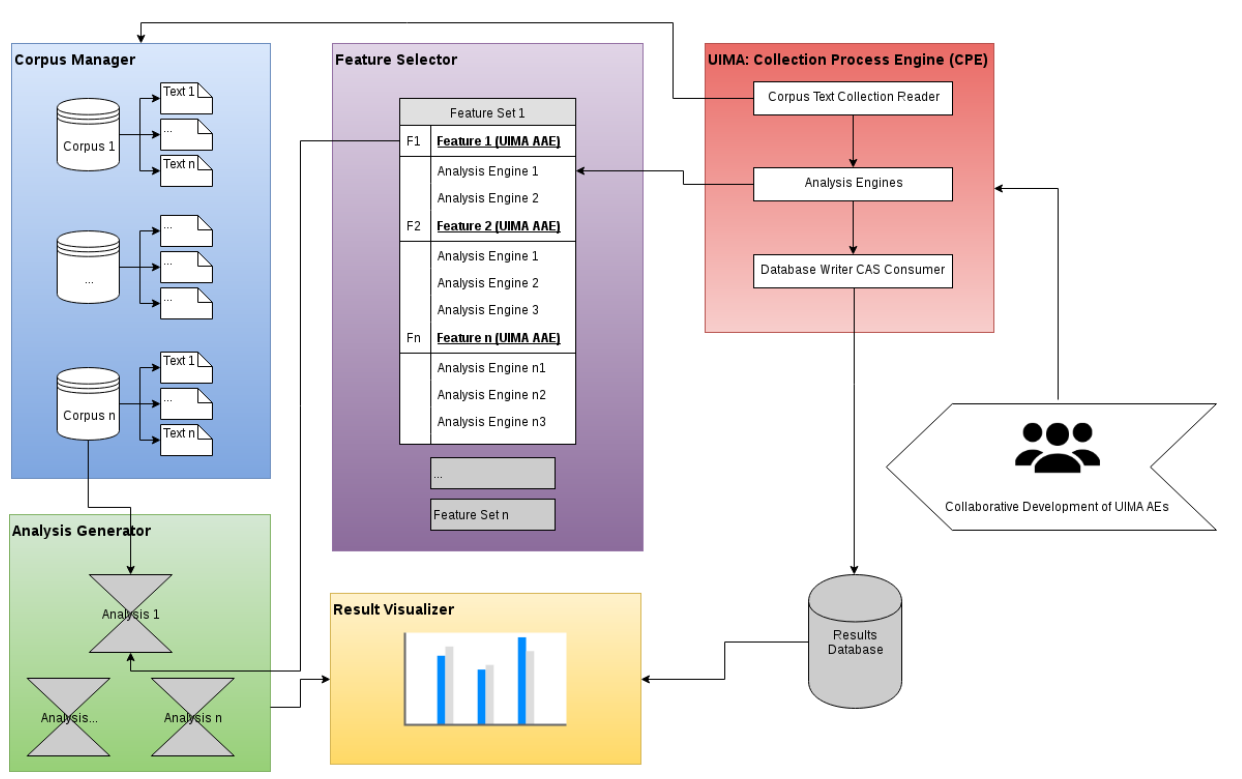
\includegraphics[scale=0.3]{images/ctap.png}
    \caption{Overview of the CTAP architecture. Source: \cite{chen2016-ctap}.}
    \label{fig:ctap}
\end{figure}

CTAP has integrated Portuguese by way of Stanza, the Stanford NLP Group's newly introduced, fully neural, end-to-end NLP pipeline that is compatible with up to 66 languages \citep{qi2020-stanza}. The LingMod Research Group has created a Java wrapper\footnote{\texttt{\url{https://github.com/lingmod-tue/stanza-java}}} around a containerized web service\footnote{\texttt{\url{https://github.com/lingmod-tue/stanza-api}}} hosting Stanza and its model binaries. This effectively lays the groundwork for supporting dozens of other languages out of the box and making CTAP a truly multilingual tool.
